\section{Dấu tam thức bậc hai}

\subsection{Đề 1}	
\Opensolutionfile{ans}[ans/ans-0-B1]
\caulc
%%%=============EX_1=============%%%
\begin{ex}%[0D7N1-1]
	Tìm khẳng định đúng trong các khẳng định sau?
	\choice
	{\True $f(x)=3x^2+2x-5$ là tam thức bậc hai}
	{$f(x)=2x-4$ là tam thức bậc hai}
	{$f(x)=3x^3+2x-1$ là tam thức bậc hai}
	{$f(x)=x^4-x^2+1$ là tam thức bậc hai}
	\loigiai{
		Theo định nghĩa tam thức bậc hai thì $f(x)=3x^2+2x-5$ là tam thức bậc hai.
	}
\end{ex}

%%%=============EX_2=============%%%
\begin{ex}%[0D7H1-2]
	Cho $f(x)=ax^2+bx+c$, $\left(a\ne 0\right)$ và $\Delta=b^2-4ac$. Xác định dấu của $\Delta$ khi $f(x)$ luôn cùng dấu với hệ số $a$ với mọi $x\in \mathbb{R}$.
	\choice
	{\True $\Delta < 0$}
	{$\Delta=0$}
	{$\Delta > 0$}
	{$\Delta \ge 0$}
	\loigiai{
		Theo định lý về dấu của tam thức bậc hai thì $f(x)$ luôn cùng dấu với hệ số $a$ với mọi $x\in \mathbb{R}$ khi $\Delta < 0$.
	}
\end{ex}

%%%=============EX_3=============%%%
\begin{ex}%[0D7H1-2]
	Cho $f(x)=x^2+4$. Khẳng định nào sau đây là đúng?
	\choice
	{\True $f(x) > 0,\forall x\in \mathbb{R}$}
	{$f(x) < 0,\forall x\in \mathbb{R}$}
	{$f(x)=0,\forall x\in \mathbb{R}$}
	{$f(x) < 0,\forall x\in \left(-\infty;-2\right)\cup \left(2;+\infty \right)$}
	\loigiai{
		\begin{itemize}
			\item {\textbf{Cách 1.}} 
			Ta có: $x^2 \ge 0,\forall x\in \mathbb{R}\Rightarrow x^2+4> 0,\forall x\in \mathbb{R}$.
			\item{\textbf{Cách 2.}}  $f(x)=x^2+4$ là tam thức bậc hai có $a=1$, $\Delta=-16< 0$.\\
			Do đó $f(x) > 0,\forall x\in \mathbb{R}$.
		\end{itemize}
	}
\end{ex}

%%%=============EX_4=============%%%
\begin{ex}%[0D7N1-1]
	Tìm tất cả các giá trị của tham số $m$ để biểu thức $f(x)=(m-2)x^2+2x-3$ là một tam thức bậc hai. 
	\choice
	{$m\in \mathbb{R}$}
	{\True $m\ne 2$}
	{$m > 2$}
	{$m < 2$}
	\loigiai{
		$f(x)=(m-2)x^2+2x-3$ là một tam thức bậc hai khi và chỉ khi: $m-2\ne 0\Leftrightarrow m\ne 2$. 
	}
\end{ex}

%%%=============EX_5=============%%%
\begin{ex}%[0D7H1-2]
	Với số thực $a$ bất kỳ, biểu thức nào sau đây luôn nhận giá trị dương?
	\choice
	{$a^2+2a-1$}
	{$a^2-2a+1$}
	{\True $a^2+a+1$}
	{$a^2+2a+1$}
	\loigiai{
		Tam thức $a^2+a+1=\left(a+\dfrac{1}{2}\right)^2+\dfrac{3}{4}>0,\,\forall x$ nên $a^2+a+1$ luôn dương với mọi $a$.
	}
\end{ex}

%%%=============EX_6=============%%%
\begin{ex}%[0D7H1-2]
	Cho $f(x)=x^2-4x+4$. Mệnh đề nào sau đây là đúng?
	\choice
	{$f(x) > 0,\forall x\in \mathbb{R}$}
	{\True $f(x) > 0,\forall x\ne 2$}
	{$f(x) > 0,\forall x\ne 4$}
	{$f(x) < 0,\forall x\in \mathbb{R}$}
	\loigiai{
		Ta có $f(x)=\left(x-2\right)^2 > 0,\forall x\ne 2$.
	}
\end{ex}

%%%=============EX_7=============%%%
\begin{ex}%[0D7N1-2]
	Nghiệm của tam thức bậc hai $f(x)=x^2-9$ là
	\choice
	{$x=-3$}
	{$x=3$}
	{\True $\hoac{&{x=3} \\
			&{x=-3}
			&}$}
	{$\hoac{&{x=0} \\
			&{x=9}
			&}$}
	\loigiai{
		Ta có $f(x)=0\Leftrightarrow x=\pm 3$.
	}
\end{ex}

%%%=============EX_8=============%%%
\begin{ex}%[0D7H1-2]
	Cho tam thức bậc hai $f(x)=x^2-2x$. Chọn khẳng định đúng.
	\choice
	{\True $f(x) < 0,\forall x\in \left(0;2\right)$}
	{$f(x) < 0,\forall x\in \mathbb{R}$}
	{$f(x) > 0,\forall x\in \mathbb{R}$}
	{$f(x) > 0,\forall x\in \left(1;+\infty \right)$}
	\loigiai{
		$f(x)=0\Leftrightarrow \hoac{&{x=0} \\
			&{x=2}
			&}$ và $a=1> 0$.\\
		Bảng xét dấu
		\begin{center}
			\begin{tikzpicture}[>=stealth]
				\tkzTabInit[nocadre=false,lgt=1.5,espcl=2,deltacl=0.6]{$x$/.7 ,$f(x)$/.7}
				{$-\infty$ , $0$ , $2$ , $+\infty$}
				\tkzTabLine{ , + , $0$ , - , $0$ , + , }
			\end{tikzpicture}
		\end{center}
		Do đó $f(x) < 0,\forall x\in \left(0;2\right)$.
	}
\end{ex}

%%%==============EX_9============%%%
\begin{ex}%[0D7H1-2]
	Bảng xét dấu sau là của tam thức bậc hai nào?
	\begin{center}
		\begin{tikzpicture}[>=stealth]
			\tkzTabInit[nocadre=false,lgt=1.5,espcl=2,deltacl=0.6]{$x$/.7 ,$f(x)$/.7}
			{$-\infty$ , $1$ , $2$ , $+\infty$}
			\tkzTabLine{ , - , $0$ , + , $0$ , - , }
		\end{tikzpicture}
	\end{center}
	\choice
	{$f(x)=-x^2-3x+2$}
	{\True $f(x)=\left(x-1\right)\left(-x+2\right)$}
	{$f(x)=x^2+3x+2$}
	{$f(x)=x^2-3x+2$}
	\loigiai{
		Dựa vào bảng xét dấu, ta có
		\begin{itemize}
			\item $f(x)$ có nghiệm là $1$ và $2$ nên loại $f(x)=-x^2-3x+2$ và $f(x)=x^2+3x+2$;
			\item $\forall x\in \left(1; 2\right),f(x) > 0$ nên $a < 0$. Do đó đáp án $f(x)=x^2-3x+2$ sai;
			\item Đáp án $f(x)=\left(x-1\right)\left(-x+2\right)$ đúng.
		\end{itemize}
	}
\end{ex}


%%%=============EX_10=============%%%
\begin{ex}%[0D7H2-1]
	Cho tam thức bậc hai $f(x)=-x^2-4x+5$. Tìm tất cả giá trị của $x$ để $f(x)\ge 0$.
	\choice
	{$x\in \left(-\infty;-1\right]\cup \left[5;+\infty \right)$}
	{$x\in \left[-1; 5\right]$}
	{\True $x\in \left[-5; 1\right]$}
	{$x\in \left(-5; 1\right)$}
	\loigiai{
		Xét tam thức $f(x)=-x^2-4x+5$. Ta có
		\begin{itemize}
			\item $a=-1< 0$;
			\item $\Delta=36> 0$ nên  tam thức $f(x)$ có hai nghiệm $x=1$ và $x=-5$.
		\end{itemize}
		Bảng xét dấu
		\begin{center}
			\begin{tikzpicture}[>=stealth]
				\tkzTabInit[nocadre=false,lgt=1.5,espcl=2,deltacl=0.6]{$x$/.7 ,$f(x)$/.7}
				{$-\infty$ , $-5$ , $1$ , $+\infty$}
				\tkzTabLine{ , - , $0$ , + , $0$ , - , }
			\end{tikzpicture}
		\end{center}
		Suy ra $f(x)\ge 0$ khi $-5\le x\le 1$.
	}
\end{ex}

%%%=============EX_11=============%%%
\begin{ex}%[0D7H1-2]
	Dấu của tam thức bậc hai $f(x)=-x^2+5x-6$ được xác định như sau
	\choice
	{$f(x) < 0$ với $2< x < 3$ và $f(x) > 0$ với $x < 2$ hoặc $x > 3$}
	{$f(x) < 0$ với $-3< x <-2$ và $f(x) > 0$ với $x <-3$ hoặc $x >-2$}
	{\True $f(x) > 0$ với $2< x < 3$ và $f(x) < 0$ với $x < 2$ hoặc $x > 3$}
	{$f(x) > 0$ với $-3< x <-2$ và $f(x) < 0$ với $x <-3$ hoặc $x >-2$}
	\loigiai{
		Xét tam thức $f(x)=-x^2+5x-6$.\\
		Ta có $\Delta=1> 0$ với hệ số $a=-1< 0$ có hai nghiệm là $x=3$ và $x=2$.\\
		Bảng xét dấu
		\begin{center}
			\begin{tikzpicture}[>=stealth]
				\tkzTabInit[nocadre=false,lgt=1.5,espcl=2,deltacl=0.6]{$x$/.7 ,$f(x)$/.7}
				{$-\infty$ , $2$ , $3$ , $+\infty$}
				\tkzTabLine{ , - , $0$ , + , $0$ , - , }
			\end{tikzpicture}
		\end{center}
		Suy ra $f(x)> 0$ khi $2< x<3$ và $f(x)<0$ khi $x<2$ hoặc $x>3$.
	}
\end{ex}

%%%=============EX_12=============%%%
\begin{ex}%[0D7N1-1]
	Tìm tất cả các giá trị của tham số $m$ để biểu thức $f(x)=\left(m-2\right)x^2+2x-3$ là một tam thức bậc hai.
	\choice
	{$m\in \mathbb{R}$}
	{\True $m\ne 2$}
	{$m > 2$}
	{$m < 2$}
	\loigiai{
		Biểu thức $f(x)=\left(m-2\right)x^2+2x-3$ là một tam thức bậc hai khi $m-2\ne 0\Leftrightarrow m\ne 2$.
	}
\end{ex}
\Closesolutionfile{ans}
\indapan{6}{ans/ans-0-B1}
\cauds
\Opensolutionfile{ans}[ans/ans-0-B1-DS]
%%%============EX_1==============%%%
\begin{ex}%[0D7N1-1]
	Các mệnh đề sau đúng hay sai?
	\choiceTF
	{$3x+7$ là tam thức bậc hai}
	{\True $-x^2+3$ là tam thức bậc hai}
	{\True $3x(x-1)$ là tam thức bậc hai}
	{$(x-1)(x+1)-x^2$ là tam thức bậc hai}
	\loigiai{
		\begin{itemchoice}
			\itemch Sai. Vì $3x+7$ không có dạng $ax^2+bx+c$.
			\itemch Đúng. Vì $-x^2+3$ nó có dạng $ax^2+bx+c$.
			\itemch Đúng. Vì $3x(x-1)=3x^2-3x$ là tam thức bậc hai.
			\itemch Sai. Vì $(x-1)(x+1)-x^2=x^2-1-x^2=1$.
		\end{itemchoice}
	}
\end{ex}
%%%==============EX_2============%%%
\begin{ex}%[0D7H1-2]
	Xét tính đúng, sai của các khẳng định sau:
	\choiceTF
	{\True $f(x)=x^2-x-2$ có $f(x) < 0$ với mọi $x\in (-1;2)$}
	{\True $f(x)=-x^2+2x-5$ có $f(x) > 0$ với mọi $x\in \mathbb{R}$}
	{\True $f(x)=-4x^2+16x-16$ có bảng xét dấu là\\
	\begin{tikzpicture}[>=stealth]
		\tkzTabInit[nocadre=false,lgt=1.5,espcl=2,deltacl=0.6]{$x$/.7 ,$f(x)$/.7}
		{$-\infty$ , $2$ , $+\infty$}
		\tkzTabLine{ , - , $0$ , - , }
\end{tikzpicture}}
	{$f(x)=-4x^2+3x-5$ có bảng xét dấu là\\
	\begin{tikzpicture}[>=stealth]
		\tkzTabInit[nocadre=false,lgt=1.5,espcl=2,deltacl=0.6]{$x$/.7 ,$f(x)$/.7}
		{$-\infty$ ,  $+\infty$}
		\tkzTabLine{ , + , }
\end{tikzpicture}}
	\loigiai{
		\begin{itemchoice}
			\itemch Đúng. Xét $f(x)=x^2-x-2$ có $a=1> 0$ và có hai nghiệm $x_1=-1;x_2=2$.\\
			Do đó, ta có bảng xét dấu sau
			\begin{center}
				\begin{tikzpicture}[>=stealth]
					\tkzTabInit[nocadre=false,lgt=1.5,espcl=2,deltacl=0.6]{$x$/.7 ,$f(x)$/.7}
					{$-\infty$ , $-1$ , $2$ , $+\infty$}
					\tkzTabLine{ , + , $0$ , - , $0$ , + , }
				\end{tikzpicture}
			\end{center}
			Vậy $f(x) < 0$ với mọi $x\in (-1;2)$.
			\itemch Đúng. Xét $f(x)=-x^2+2x-5$ có $\heva{&a=1> 0\\&\Delta'=-4< 0}$ nên $f(x) > 0$ với mọi $x\in \mathbb{R}$.
			\itemch Đúng. Ta có $-4x^2+16x-16=0\Leftrightarrow x=2$.\\
			Do đó, ta có bảng xét dấu sau
			\begin{center}
				\begin{tikzpicture}[>=stealth]
					\tkzTabInit[nocadre=false,lgt=1.5,espcl=2,deltacl=0.6]{$x$/.7 ,$f(x)$/.7}
					{$-\infty$ , $2$ , $+\infty$}
					\tkzTabLine{ , - , $0$ , - , }
				\end{tikzpicture}
			\end{center}
			\itemch Sai. Ta có $-4x^2+3x-5=0$ vô nghiệm. Bảng xét dấu
			\begin{center}
				\begin{tikzpicture}[>=stealth]
					\tkzTabInit[nocadre=false,lgt=1.5,espcl=2,deltacl=0.6]{$x$/.7 ,$f(x)$/.7}
					{$-\infty$ ,$+\infty$}
					\tkzTabLine{ , - , }
				\end{tikzpicture}
			\end{center}
		\end{itemchoice}
	}
	\end{ex}
%%%==============EX_3============%%%
\begin{ex}%[0D7H1-3]
	Cho đồ thị hàm số bậc hai $y=f(x)$ và $y=g(x)$.
	\begin{center}
		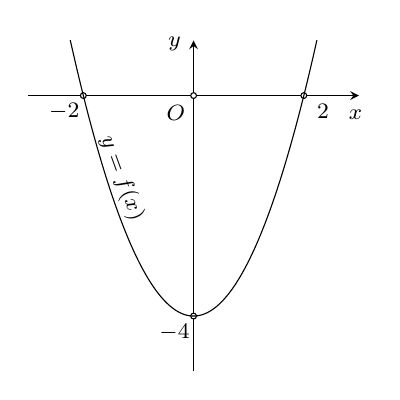
\begin{tikzpicture}[line cap=butt,line join=miter,>=stealth,font=\footnotesize,scale=.7]
			\tikzset{declare function={xmin=-3;xmax=3;ymin=-5;ymax=1;
					f(\x)=1*(\x)^2-4;
				},
				smooth,samples=450
			}
			\draw[->] (xmin,0)--(xmax,0) node[shift={(-100:7pt)}]{$ x $};
			\draw[->] (0,ymin)--(0,ymax) node[shift={(190:7pt)}]{$ y $};
			\fill (0,0) node[shift={(225:9pt)}]{$ O $};
			\draw[fill=white] (0,0) circle (1.5pt) 
			(-2,0)node[shift={(-140:9pt)}]{$-2$} circle (1.5pt)
			(2,0)node[shift={(-40:9pt)}]{$2$} circle (1.5pt)
			(0,-4)node[shift={(-140:9pt)}]{$-4$} circle (1.5pt);
			\node[rotate=-70] at (-1.3,-1.5){$y=f(x)$};
			\clip (xmin,ymin) rectangle (xmax,ymax);
			\draw  plot[domain=xmin:xmax] (\x, {f(\x)});
		\end{tikzpicture}\hspace{2cm}
	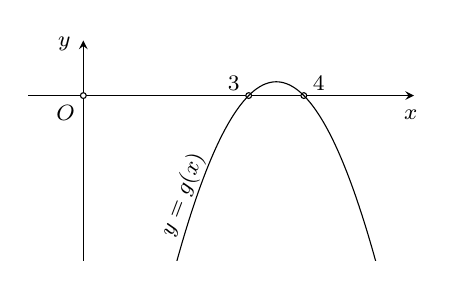
\begin{tikzpicture}[line cap=butt,line join=miter,>=stealth,font=\footnotesize,scale=.7]
		\tikzset{declare function={xmin=-1;xmax=6;ymin=-3;ymax=1;
				f(\x)=-1*(\x)^2+7*(\x)-12;
			},
			smooth,samples=450
		}
		\draw[->] (xmin,0)--(xmax,0) node[shift={(-100:7pt)}]{$ x $};
		\draw[->] (0,ymin)--(0,ymax) node[shift={(190:7pt)}]{$ y $};
		\fill (0,0) node[shift={(225:9pt)}]{$ O $};
		\draw[fill=white] (0,0) circle (1.5pt) 
		(3,0)node[shift={(140:7pt)}]{$3$} circle (1.5pt)
		(4,0)node[shift={(40:7pt)}]{$4$} circle (1.5pt);
		\node[rotate=69] at (1.8,-1.8){$y=g(x)$};
		\clip (xmin,ymin) rectangle (xmax,ymax);
		\draw  plot[domain=xmin:xmax] (\x, {f(\x)});
	\end{tikzpicture}
	\end{center}
	Các mệnh đề sau đúng hay sai?
		\choiceTF
		{\True Đồ thị hàm số $y=f(x)$ cắt trục hoành tại hai điểm $(-2;0)$ và $(2;0)$}
		{\True Đồ thị hàm số $y=g(x)$ cắt trục hoành tại hai điểm $(3;0)$ và $(4;0)$}
		{Tam thức bậc hai $f(x)$ có bảng xét dấu\\\begin{tikzpicture}[>=stealth]
					\tkzTabInit[nocadre=false,lgt=1.5,espcl=2,deltacl=0.6]{$x$/.7 ,$f(x)$/.7}
					{$-\infty$,$-2$, $2$ ,$+\infty$}
					\tkzTabLine{ , - ,$0$, + ,$0$, - ,}
				\end{tikzpicture}}
		{Tam thức bậc hai $g(x)$ có bảng xét dấu \\\begin{tikzpicture}[>=stealth]
				\tkzTabInit[nocadre=false,lgt=1.5,espcl=2,deltacl=0.6]{$x$/.7 ,$g(x)$/.7}
				{$-\infty$,$3$, $4$ ,$+\infty$}
				\tkzTabLine{ , + ,$0$, - ,$0$, + ,}
		\end{tikzpicture}}
	\loigiai{
				\begin{itemchoice}
					\itemch Đúng. Đồ thị hàm số $y=f(x)$ cắt trục hoành tại hai điểm $(-2;0)$ và $(2;0)$.
					\itemch Đúng. Đồ thị hàm số $y=g(x)$ cắt trục hoành tại hai điểm $(3;0)$ và $(4;0)$.
					\itemch Sai. Đồ thị hàm số $y=f(x)$ cắt trục hoành tại hai điểm $(-2;0)$ và $(2;0)$ nên tam
					thức bậc hai $f(x)$ có hai nghiệm là $x_1=-2,x_2=2$. Đồ thị có bề lõm quay lên nên hệ số $a > 0$. Do đó, ta có bảng xét dấu sau
					\begin{center}
						\begin{tikzpicture}[>=stealth]
							\tkzTabInit[nocadre=false,lgt=1.5,espcl=2,deltacl=0.6]{$x$/.7 ,$g(x)$/.7}
							{$-\infty$,$-2$, $2$ ,$+\infty$}
							\tkzTabLine{ , + ,$0$, - ,$0$, + ,}
						\end{tikzpicture}
					\end{center}
					\itemch Sai. Quan sát đồ thị hàm số $y=g(x)$, ta thấy $(3;0)$ và $(4;0)$ nên tam
					thức bậc hai $g(x)$ có hai nghiệm là $x_1=3,x_2=4$.
					\begin{center}
						\begin{tikzpicture}[>=stealth]
							\tkzTabInit[nocadre=false,lgt=1.5,espcl=2,deltacl=0.6]{$x$/.7 ,$g(x)$/.7}
							{$-\infty$,$3$, $4$ ,$+\infty$}
							\tkzTabLine{ , - ,$0$, + ,$0$, - ,}
						\end{tikzpicture}
					\end{center}
				\end{itemchoice}
			}
		\end{ex}
%%%==============EX_4============%%%
\begin{ex}%[0D7H1-3]
	Cho biểu thức $f(x)=\dfrac{x-3}{x^2+7x+6}$. Các mệnh đề sau đúng hay sai?
	\choiceTF
	{$f(x)=0\Leftrightarrow \hoac{&{x=-1} \\
			&{x=-6}
			&}$}
	{với $x\in (-\infty;-6)\cup (-1;3)$ thì $f(x) > 0$}
	{với $x\in (-6;-1)\cup (3;+\infty)$ thì $f(x) < 0$}
	{\True Bảng xét dấu của biểu thức là\\
	\begin{tikzpicture}[>=stealth]
		\tkzTabInit[nocadre=false,lgt=3]{$x$/.7 ,$x-3$/.7,$x^2+7x+6$/.7,$f(x)$/.7}
		{$-\infty$,$-6$, $-1$ ,$3$ ,$+\infty$}
		\tkzTabLine{ , - ,t, - ,t, - ,$0$, + ,}
		\tkzTabLine{ , + ,$0$, - ,$0$, + ,t, + ,}
		\tkzTabLine{ , - ,d, + ,d, - ,$0$, + ,}
\end{tikzpicture}}
	\loigiai{
		Bảng xét dấu
		\begin{center}
			\begin{tikzpicture}[>=stealth]
				\tkzTabInit[nocadre=false,lgt=3]{$x$/.7 ,$x-3$/.7,$x^2+7x+6$/.7,$f(x)$/.7}
				{$-\infty$,$-6$, $-1$ ,$3$ ,$+\infty$}
				\tkzTabLine{ , - ,t, - ,t, - ,$0$, + ,}
				\tkzTabLine{ , + ,$0$, - ,$0$, + ,t, + ,}
				\tkzTabLine{ , - ,d, + ,d, - ,$0$, + ,}
			\end{tikzpicture}
		\end{center}
		\begin{itemchoice}
			\itemch Sai. Ta có $f(x)=0\Rightarrow x-3=0\Leftrightarrow x=3$ thỏa điều kiện $x^2+7x+6\neq 0$.
			\itemch Sai. Dựa vào bảng xét dấu, ta có $f(x)>0$ khi $x\in(-6;-1)\cup(3;+\infty)$.
			\itemch Sai. Dựa vào bảng xét dấu, ta có $f(x)<0$ khi $x\in(-\infty;-6)\cup(-1;3)$.
			\itemch Đúng. 
		\end{itemchoice}
		
	}
\end{ex}
\Closesolutionfile{ans}
\indapan{3}{ans/ans-0-B1-DS}
\Opensolutionfile{ans}[ans/ans-0-B1-KQ]
\caukq
%%%==============EX_1============%%%
\begin{ex}%[0D7V2-6]
	Tìm số nguyên âm $m$ lớn nhất  sao cho $-x^2+2(m+1)x-m^2+m < 0$ với mọi $x\in \mathbb{R}$.
	\shortans{$-1$}
	\loigiai{
		Xét tam thức bậc hai $f(x)=-x^2+2(m+1)x-m^2+m$ có \[\Delta '=\left(m+1\right)^2-\left(-1\right).\left(-m^2+m\right)=3m+1\text{ và }a=-1< 0.\]
		Để $f(x) < 0$ với mọi $x\in \mathbb{R}$ thì $\Delta '=3m+1< 0$ suy ra $m < \dfrac{-1}{3}$.
	}
\end{ex}
%%%==============EX_2============%%%
\begin{ex}%[0D7V2-3]
	Giải bất phương trình $\left(x^2-3x+2\right)\left(-x^2+5x-6\right)\ge 0$ ta được tập nghiệm $S=[a;b]$. Tính giá trị của biểu thức $a+3b$.
	\shortans{$10$}
	\loigiai{
		Tam thức bậc hai $f(x)=x^2-3x+2$ có $a=1> 0$ và có hai nghiệm $x_1=1;x_2=2$.\\
		Tam thức bậc hai $g(x)=-x^2+5x-6$ có $a=-1< 0$ và có hai nghiệm $x_1=2;x_2=3$
		Ta có bảng xét dấu sau	
		\begin{center}
			\begin{tikzpicture}[>=stealth]
				\tkzTabInit[nocadre=false,lgt=3]{$x$/.7 ,$x^2-3x+2$/.7,$-x^2+5x-6$/.7,$f(x)$/.7}
				{$-\infty$,$1$, $2$ ,$3$ ,$+\infty$}
				\tkzTabLine{ , + ,$0$, - ,$0$, + ,t, + ,}
				\tkzTabLine{ , - ,t, - ,$0$, + ,$0$, - ,}
				\tkzTabLine{ , - ,$0$, + ,$0$, + ,$0$, - ,}
			\end{tikzpicture}
		\end{center}	
		Suy ra $f(x)\cdot g(x)\ge 0$ khi $x\in [1;3]$.
		Vậy  giá trị của biểu thức $a+3b=1+3\cdot 3=10$.
	}
\end{ex}
%%%==============EX_3============%%%
\begin{ex}%[0D7V2-6]
	Có bao nhiêu giá trị nguyên của tham số $m$ thuộc đoạn $\left[-20;30\right]$ để bất phương trình $x^2+2mx+m-2< 0$ nghiệm đúng với mọi $x\in (1;2)$?
	\shortans{$20$}
	\loigiai{
		Tam thức bậc hai $f(x)=x^2+2mx+m-2$ có \[\Delta'=m^2-m+2=\left(m-\dfrac{1}{2} \right)^2+\dfrac{7}{4} \ge \dfrac{7}{4} > 0,\,\forall m\in \mathbb{R}.\]
		Do đó $f(x)$ có hai nghiệm phân biệt $x_1, x_2\,\left(x_1 < x_2 \right)$ với mọi $m\in \mathbb{R}$.\\
		Để $f(x) < 0$ với mọi $x\in (1;2)$ thì $x_1 \le 1< 2\le x_2$ \[\Leftrightarrow \heva{&f(1)\leq 0\\&f(2)\leq 0}\Leftrightarrow\heva{&3m-2\leq 0\\&5m+2\leq 0}\Rightarrow m\leq -\dfrac{2}{5}.\]
		Vậy có $20$ giá trị nguyên của tham số $m$ thuộc đoạn $\left[-20;30\right]$ thỏa mãn yêu cầu bài toán.
	}
\end{ex}
%%%==============EX_4============%%%
\begin{ex}%[0D7H2-6]
	Có bao nhiêu giá trị nguyên của tham số $m$ thuộc đoạn $\left[-10;5\right]$ để phương trình $x^2-(m+1)x+3m-5=0$ có hai nghiệm phân biệt?
	\shortans{$13$}
	\loigiai{
		Ta có $\Delta=[-(m+1)]^2-4\cdot 1\cdot (3m-5)=m^2-10m+21$.\\
		Để phương trình $x^2-(m+1)x+3m-5=0$ có hai nghiệm phân biệt thì \[\Delta > 0\text{ hay } m^2-10m+21> 0.\]
		Tam thức bậc hai $m^2-10m+21$ có $a=1> 0$ và có hai nghiệm $m_1=3,m_2=7$.\\
		Do đó, $m^2-10m+21> 0$ khi $m\in (-\infty;3)\cup (7;+\infty)$.\\
		Mà $m\in \mathbb{Z}$ và $m\in \left[-10;5\right]$ nên có $13$ giá trị nguyên của tham số $m$ thỏa mãn.
	}
\end{ex}
%%%==============EX_5============%%%
\begin{ex}%[0D7V2-7]
	Một chú thỏ đen chạy đuổi theo một chú thỏ trắng ở vị trí cách nó $100$~(m). Biết rằng, quãng đường chú thỏ đen chạy được biểu thị bởi công thức $s(t)=8t+5t^2$~(m), trong đó $t$ (giây) là thời gian tính từ thời điểm chú thỏ đen bắt đầu chạy, và chú thỏ trắng chạy với vận tốc không đổi là $3$~(m/s). Hỏi bắt đầu từ giá trị nguyên $t$ nào thì chú thỏ đen chạy trước chú thỏ trắng?
	\shortans{$5$}
	\loigiai{
		Giả sử vị trí ban đầu của chú thỏ đen là $s=0$~(m) và thời điểm ban đầu là $t=0$ (giây).\\
		Quãng đường của chú thỏ trắng chạy được tại thời điểm $t$ là $f(t)=100+3t$~(m).\\
		Để chú thỏ đen chạy trước chú thỏ trắng thì \[s(t) > f(t)\text{ hay }8t+5t^2 > 100+3t\Leftrightarrow 5t^2+5t-100> 0\Rightarrow t\in (4;+\infty) (\text{vì }t>0).\]
		Vậy bắt đầu giây thứ $5$ thì chú thỏ đen chạy trước chú thỏ trắng.
	}
\end{ex}
%%%==============EX_6============%%%
\begin{ex}%[0D7V2-6]
	Có bao nhiêu giá trị nguyên của tham số $m$, hàm số $y=\sqrt{x^2-2mx+m-1}$ có tập xác định là $\mathbb{R}$?
	\shortans{$0$}
	\loigiai{
		Để hàm số $y=\sqrt{x^2-2mx+m-1}$ có tập xác định là $\mathbb{R}$ thì \[x^2-2mx+m-1\ge 0,\,\forall x\in \mathbb{R}\Leftrightarrow\heva{&{a > 0} \\
			&{\Delta \le 0}&}\Leftrightarrow\heva{&1>0\\&m^2-m+1\leq 0\;(*)}.\]
		Vì $\left(m-\dfrac{1}{2}\right)^2+\dfrac{3}{4}>0,\,\forall x$ nên (*) vô nghiệm.\\
		Vậy không tồn tại giá trị của tham số $m$ để thoả mãn yêu cầu bài toán.
	}
\end{ex}
\Closesolutionfile{ans}
\indapan{6}{ans/ans-0-B1-KQ}
\newpage
\subsection{Đề 2}	
\Opensolutionfile{ans}[ans/ans-0-B1]
\caulc
%%%==============EX_1============%%%
\begin{ex}%[0D7H1-2]
	Tam thức bậc hai $f(x)=x^2-12x-13$ nhận giá trị không âm khi và chỉ khi
	\choice
	{$x\in \left(-1;13\right)$}
	{$x\in \mathbb{R}\setminus \left[-1;13\right]$}
	{$x\in \left[-1;13\right]$}
	{\True $x\in \left(-\infty;-1\right]\cup \left[13;+\infty \right)$}
	\loigiai{
		$f(x)=0\Leftrightarrow x^2-12x-13=0\Leftrightarrow \hoac{&{x=-1} \\
			&{x=13.}
			&}$\\
		Bảng xét dấu của $f(x)$
		\begin{center}
			\begin{tikzpicture}[>=stealth]
				\tkzTabInit[nocadre=false,lgt=1.5,espcl=2,deltacl=0.6]{$x$/.7 ,$f(x)$/.7}
				{$-\infty$ , $-1$ , $13$ , $+\infty$}
				\tkzTabLine{ , + , $0$ , - , $0$ , + , }
			\end{tikzpicture}
		\end{center}		
		Vậy $f(x)\ge 0\Leftrightarrow x\in \left(-\infty;-1\right]\cup \left[13;+\infty \right)$.
	}
\end{ex}
%%%==============EX_2============%%%
\begin{ex}%[0D7H1-2]
	Cho tam thức $f(x)=ax^2+bx+c\left(a\ne 0\right)$, $\Delta=b^2-4ac$. Ta có $f(x)\le 0$ khi và chỉ khi
	\choice
	{\True $\heva{&{a < 0} \\
			&{\Delta \le 0}
			&}$}
	{$\heva{&{a < 0} \\
			&{\Delta \ge 0}
			&}$}
	{$\heva{&{a\le 0} \\
			&{\Delta < 0}
			&}$}
	{$\heva{&{a > 0} \\
			&{\Delta \le 0}
			&}$}
	\loigiai{
		Ta có $f(x)\le 0$ khi và chỉ khi $\heva{&{a < 0} \\
			&{\Delta \le 0.}
			&}$
	}
\end{ex}
%%%==============EX_3============%%%
\begin{ex}%[0D7H1-2]
	Các giá trị của $m$ để tam thức $f(x)=x^2-\left(m+2\right)x+8m+1$ có hai nghiệm phân biệt là
	\choice
	{$m > 0$}
	{$m\le 0$ hay $m\ge 28$}
	{\True $m < 0$ hay $m > 28$}
	{$0< m < 28$}
	\loigiai{
		Để tam thức $f(x)$ có hai nghiệm phân biệt thì
		\[\Leftrightarrow \Delta > 0\Leftrightarrow \left(m+2\right)^2-4\cdot\left(8m+1\right) > 0\Leftrightarrow m^2-28m > 0\Leftrightarrow m < 0 \text{ hay } m > 28.
		\]
	}
\end{ex}
%%%==============EX_4============%%%
\begin{ex}%[0D7H1-2]
	Tam thức bậc hai $f(x)=-x^2+3x-2$ nhận giá trị không âm khi và chỉ khi
	\choice
	{$x\in \left(-\infty;1\right]\cup \left[2;+\infty \right)$}
	{\True $x\in \left[1;2\right]$}
	{$x\in \left(1;2\right)$}
	{$x\in \left(-\infty;1\right)\cup \left(2;+\infty \right)$}
	\loigiai{
		\[f(x)=0\Leftrightarrow-x^2+3x-2=0\Leftrightarrow \hoac{&{x=1} \\
			&{x=2.}
			&}
		\]
		Bảng xét dấu $f(x)$
		\begin{center}
			\begin{tikzpicture}[>=stealth]
				\tkzTabInit[nocadre=false,lgt=1.5,espcl=2,deltacl=0.6]{$x$/.7 ,$f(x)$/.7}
				{$-\infty$ , $1$ , $2$ , $+\infty$}
				\tkzTabLine{ , - , $0$ , + , $0$ , - , }
			\end{tikzpicture}
		\end{center}	
		Vậy $f(x)\ge 0\Leftrightarrow x\in \left[1;2\right]$.
	}
\end{ex}
%%%==============EX_5============%%%
\begin{ex}%[0D7H1-3]
	Bảng xét dấu sau là của biểu thức nào?
	\begin{center}
		\begin{tikzpicture}[>=stealth]
			\tkzTabInit[nocadre=false,lgt=1.5,espcl=2,deltacl=0.6]{$x$/.7 ,$f(x)$/.7}
			{$-\infty$ , $-2$ , $-1$ , $+\infty$}
			\tkzTabLine{ , - , $0$ , + , $0$ , - , }
		\end{tikzpicture}
	\end{center}
	\choice
	{$f(x)=(x-1)(x+2)$}
	{$f(x)=(x+1)(x+2)$}
	{$f(x)=x^2-3x+2$}
	{\True $f(x)=-x^2-3x-2$}
	\loigiai{
		Dựa vào bảng xét dấu, ta thấy
		\begin{itemize}
			\item $f(x)=0$ có hai nghiệm $x=-1$ và $x=-2$.
			\item $a<0$.
		\end{itemize}
	Do đó bảng xét dấu trên là của tam thức $f(x)=-x^2-3x-2$.
	}
\end{ex}
%%%==============EX_6============%%%
\begin{ex}%[0D7H1-2]
	Cho biểu thức $f(x)=x^2 \left(x^2-4\right)$ có bảng xét dấu như sau
	\begin{center}
		\begin{tikzpicture}[>=stealth]
			\tkzTabInit[nocadre=false,lgt=1.5,espcl=2,deltacl=0.6]{$x$/.7 ,$f(x)$/.7}
			{$-\infty$ , $-2$ , $0$, $2$ , $+\infty$}
			\tkzTabLine{ , ? , $0$ , ? , $0$ , ? ,$0$ , ? , }
		\end{tikzpicture}
	\end{center}
	Dấu trong các dấu chấm hỏi theo thứ tự từ trái sang phải là
	\choice
	{\True $+,-,-,+$}
	{$+,-,+,-$}
	{$-,+,-,+$}
	{$+,+,-,+$}
	\loigiai{
		Ta có $f(x)=0\Leftrightarrow \hoac{&{x=0} \\
			&{x=\pm 2.}
			&}$\\
		 Ta có bảng xét dấu $f(x)=x^2\left(x^2-4\right)$ như sau
		 \begin{center}
		 	\begin{tikzpicture}[>=stealth]
		 		\tkzTabInit[nocadre=false,lgt=1.5,espcl=2,deltacl=0.6]{$x$/.7 ,$f(x)$/.7}
		 		{$-\infty$ , $-2$ , $0$, $2$ , $+\infty$}
		 		\tkzTabLine{ , + , $0$ , - , $0$ , - ,$0$ , + , }
		 	\end{tikzpicture}
		 \end{center}
	 Do đó các dấu chấm hỏi theo thứ tự từ trái sang phải là $+,-,-,+$.
	}
\end{ex}
%%%==============EX_7============%%%
\begin{ex}%[0D7H1-3]
	Cho $f(x)=ax^2+b x+c\, \left(a\ne 0\right)$ có bảng xét dấu dưới đây
	\begin{center}
		\begin{tikzpicture}[>=stealth]
			\tkzTabInit[nocadre=false,lgt=1.5,espcl=2,deltacl=0.6]{$x$/.7 ,$f(x)$/.7}
			{$-\infty$ , $x_1$, $x_2$ , $+\infty$}
			\tkzTabLine{ , + , $0$ , - , $0$ , + , }
			\path ($(L1)!.5!(L2)$)node{$0$};
		\end{tikzpicture}
	\end{center}
	Hỏi mệnh đề nào dưới đây đúng?
	\choice
	{\True $a > 0,b < 0,c > 0$}
	{$a < 0,b < 0,c > 0$}
	{$a > 0,b > 0,c > 0$}
	{$a > 0,b < 0,c < 0$}
	\loigiai{
		\begin{itemize}
			\item Tại $x=0$ thì $f(0)=c > 0$.
			\item Trong khoảng hai nghiệm $\left(x_1;x_2 \right)$, $f(x)$ mang dấu \lq\lq$-$\rq\rq\, nên $a > 0$.
			\item Phương trình $f(x)=0$ có hai nghiệm $x_1, x_2$ thỏa mãn $0< x_1 < x_2$ $\Rightarrow x_1+x_2 > 0$.
			\item Theo định lý Vi-ét $x_1+x_2=\dfrac{-b}{a}$ nên $\dfrac{-b}{a} > 0\Rightarrow b < 0$.
		\end{itemize}
		
	}
\end{ex}
%%%==============EX_8============%%%
\begin{ex}%[0D7V1-4]
	Cho biểu thức $f(x)=\dfrac{\left(x^2-4x+4\right)\left(x+3\right)}{5x}$. Trong khoảng $\left(0;2\right)$, $f(x)$ mang dấu gì?
	\choice
	{\True dương}
	{âm}
	{không dương}
	{không âm}
	\loigiai{
		Ta có 
		\begin{itemize}
			\item $x^2-4x+4=0\Leftrightarrow x=2$.
			\item $x+3=0\Leftrightarrow x=-3$.
			\item $5x=0\Leftrightarrow x=0$.
		\end{itemize}
		Bảng xét dấu
		\begin{center}
			\begin{tikzpicture}[>=stealth]
				\tkzTabInit[nocadre=false,lgt=3]{$x$/.7 ,$x^2-4x+4$/.7,$x+3$/.7,$5x$/.7,$f(x)$/.7}
				{$-\infty$,$-3$, $0$ ,$2$ ,$+\infty$}
				\tkzTabLine{ , + ,t, + ,t, + ,$0$, + ,}
				\tkzTabLine{ , - ,$0$, + ,t, + ,t, + ,}
				\tkzTabLine{ , - ,t, - ,$0$, + ,t, + ,}
				\tkzTabLine{ , + ,$0$, - ,$0$, + ,$0$, +,}
			\end{tikzpicture}
		\end{center}
	Từ bảng xét dấu, ta thấy trong khoảng $\left(0;2\right)$, $f(x)$ mang dấu dương.
	}
\end{ex}
%%%=============EX_9=============%%%
\begin{ex}%[0D7H1-2]
	Tam thức bậc hai $f(x)=x^2-3x-4$ âm khi
	\choice
	{$x\in \left(-\infty;-1\right]\cup \left[4;+\infty \right)$}
	{$x\in \left[-4;2\right]$}
	{\True $\left(-1;4\right)$}
	{$x\in \left(-\infty;-4\right]\cup \left[1;+\infty \right)$}
	\loigiai{
		Ta có $x^2-3x-4< 0\Leftrightarrow-1< x < 4$.
	}
\end{ex}
%%%==============EX_10============%%%
\begin{ex}%[0D7H1-2]
	Với số thực $x$ bất kì, biểu thức nào sau đây luôn nhận giá trị dương?
	\choice
	{$x^2-2x+1$}
	{$x^2+2x+1$}
	{\True $x^2+x+1$}
	{$x^2+x-1$}
	\loigiai{
		Xét biểu thức $f(x)=x^2+x+1$ có $\heva{&{a=1> 0} \\
			&{\Delta=1^2-4\cdot 1=-3< 0}
			&}$ $\Rightarrow f(x) > 0$, $\forall x\in \mathbb{R}$.
	}
\end{ex}
%%%==============EX_11============%%%
\begin{ex}%[0D7H1-3]
	Bảng xét dấu sau của tam thức bậc hai nào?
	\begin{center}
		\begin{tikzpicture}[>=stealth]
			\tkzTabInit[nocadre=false,lgt=1.5,espcl=2,deltacl=0.6]{$x$/.7 ,$f(x)$/.7}
			{$-\infty$ , $-3$ , $2$ , $+\infty$}
			\tkzTabLine{ ,- , $0$ , + ,$0$ , - , }
		\end{tikzpicture}
	\end{center}
	\choice
	{$f(x)=x^2-x-6$}
	{\True $f(x)=-x^2-x+6$}
	{$f(x)=-x^2+x+6$}
	{$f(x)=x^2+x-6$}
	\loigiai{
		Từ bảng xét dấu ta thấy hệ số của $x^2$ âm
		và $f(x)=0$ có 2 nghiệm $x=-3$, $x=2$.
	}
\end{ex}
%%%==============EX_12============%%%
\begin{ex}%[0D7H2-1]
	Cho bất phương trình $x^2+bx+c > 0$. Tìm tập nghiệm $S$ của bất phương trình đó biết rằng $b^2-4c < 0$.
	\choice
	{$S=\left\{-\dfrac{b}{2} \right\}$}
	{$S={\bf \mathbb{R}}\setminus \left\{-\dfrac{b}{2} \right\}$}
	{\True $S={\bf \mathbb{R}}$}
	{$S=\varnothing$}
	\loigiai{
		Ta có $b^2-4c < 0\Rightarrow \heva{&{a=1> 0} \\
			&{\Delta < 0}}\Rightarrow x^2+bx+c > 0$, $\forall x\in {\bf \mathbb{R}}\Rightarrow S={\bf \mathbb{R}}$.
	}
\end{ex}
\Closesolutionfile{ans}
\indapan{6}{ans/ans-0-B1}
\cauds
\Opensolutionfile{ans}[ans/ans-0-B1-DS]
%%%==============EX_1============%%%
\begin{ex}%[0D7H1-2]
	Các mệnh đề sau đúng hay sai?
	\choiceTF
	{\True $f(x)=3x^2-2x-1$ có $f(x) > 0,\forall x\in \left(-\infty;-\dfrac{1}{3} \right)\cup (1;+\infty)$}
	{$f(x)=-x^2+2x-1$ có $f(x) < 0,\forall x\in \mathbb{R}$}
	{\True $f(x)=-4x^2+12x-5$ có $f(x) > 0,\forall x\in \left(\dfrac{1}{2};\dfrac{5}{2} \right)$}
	{$f(x)=3x^2-2x+8$ có $f(x) < 0,\forall x\in \mathbb{R}\setminus \{1\}$}
	\loigiai{
		\begin{itemchoice}
			\itemch Đúng. $f(x)=0\Leftrightarrow x=1,x=-\dfrac{1}{3}$.\\
			Bảng xét dấu
			\begin{center}
				\begin{tikzpicture}[>=stealth]
					\tkzTabInit[nocadre=false,lgt=1.5,espcl=2,deltacl=0.6]{$x$/.7 ,$f(x)$/.7}
					{$-\infty$ , $-\tfrac{1}{3}$ , $1$ , $+\infty$}
					\tkzTabLine{ ,+ , $0$ , - ,$0$ , + , }
				\end{tikzpicture}
			\end{center}
			Vậy $f(x) > 0,\forall x\in \left(-\infty;-\dfrac{1}{3} \right)\cup (1;+\infty);f(x) < 0,\forall x\in \left(-\dfrac{1}{3};1\right)$.
			\itemch Sai. $f(x)=0\Leftrightarrow x=1$.\\
			Bảng xét dấu
			\begin{center}
				\begin{tikzpicture}[>=stealth]
					\tkzTabInit[nocadre=false,lgt=1.5,espcl=2,deltacl=0.6]{$x$/.7 ,$f(x)$/.7}
					{$-\infty$ , $1$ , $+\infty$}
					\tkzTabLine{ ,- ,$0$, -,}
				\end{tikzpicture}
			\end{center}
			Vậy $f(x) < 0,\forall x\in \mathbb{R}\setminus \{1\}$.
			\itemch Đúng. $f(x)=0\Leftrightarrow x=\dfrac{5}{2}, x=\dfrac{1}{2}$.\\
			Bảng xét dấu
			\begin{center}
				\begin{tikzpicture}[>=stealth]
					\tkzTabInit[nocadre=false,lgt=1.5,espcl=2,deltacl=0.6]{$x$/.7 ,$f(x)$/.7}
					{$-\infty$ , $\tfrac{1}{2}$ , $\tfrac{5}{2}$ , $+\infty$}
					\tkzTabLine{ ,- , $0$ , + ,$0$ , - , }
				\end{tikzpicture}
			\end{center}
			Vậy $f(x) > 0,\forall x\in \left(\dfrac{1}{2};\dfrac{5}{2} \right);f(x) < 0,\forall x\in \left(-\infty;\dfrac{1}{2} \right)\cup \left(\dfrac{5}{2};+\infty \right)$.
			\itemch Sai. Tam thức $f(x)$ có $\heva{&a=3>0\\&\Delta'=-23<0}\Rightarrow f(x)>0,\,\forall x$.
		\end{itemchoice}
	}
	\end{ex}
	%%%==============EX_2============%%%
	\begin{ex}%[0D7H2-1]
		Các mệnh đề sau đúng hay sai?
		\choiceTF
		{$7x^2-4x-3< 0\Leftrightarrow x\in \left(-\infty;-\dfrac{3}{7} \right)\cup \left(1;+\infty \right)$}
		{$-x^2+6x-9\ge 0\Leftrightarrow x\in \mathbb{R}$}
		{\True $-5x^2+4x+12< 0\Leftrightarrow x\in \left(-\infty;-\dfrac{6}{5} \right)\cup (2;+\infty)$}
		{\True $3x^2-4x+4\ge 0\Leftrightarrow x\in \mathbb{R}$}
		\loigiai{
			\begin{itemchoice}
				\itemch Sai. $7x^2-4x-3=0\Leftrightarrow x=1$ hoặc $x=-\dfrac{3}{7}$.\\
				Bảng xét dấu
				\begin{center}
					\begin{tikzpicture}[>=stealth]
						\tkzTabInit[nocadre=false,lgt=1.5,espcl=2,deltacl=0.6]{$x$/.7 ,$f(x)$/.7}
						{$-\infty$ , $-\tfrac{3}{7}$ , $1$ , $+\infty$}
						\tkzTabLine{ ,+ , $0$ , - ,$0$ , + , }
					\end{tikzpicture}
				\end{center}
				Ta có $7x^2-4x-3< 0\Leftrightarrow x\in \left(-\dfrac{3}{7};1\right)$.\\
				Vậy tập nghiệm bất phương trình là $S=\left(-\dfrac{3}{7};1\right)$.
				\itemch Sai. $-x^2+6x-9=0\Leftrightarrow x=3$.\\
				Bảng xét dấu
				\begin{center}
					\begin{tikzpicture}[>=stealth]
						\tkzTabInit[nocadre=false,lgt=1.5,espcl=2,deltacl=0.6]{$x$/.7 ,$f(x)$/.7}
						{$-\infty$ , $3$ , $+\infty$}
						\tkzTabLine{ ,- , $0$ , - , }
					\end{tikzpicture}
				\end{center}
				Ta có $-x^2+6x-9\ge 0\Leftrightarrow x\in \{3\}$.
				Vậy tập nghiệm bất phương trình là $S=\{3\}$.
				\itemch Đúng. $-5x^2+4x+12=0\Leftrightarrow x=2$ hoặc $x=-\dfrac{6}{5}$.\\
				Bảng xét dấu
				\begin{center}
					\begin{tikzpicture}[>=stealth]
						\tkzTabInit[nocadre=false,lgt=1.5,espcl=2,deltacl=0.6]{$x$/.7 ,$f(x)$/.7}
						{$-\infty$ , $-\tfrac{6}{5}$ , $2$ , $+\infty$}
						\tkzTabLine{ ,- , $0$ , + ,$0$ , - , }
					\end{tikzpicture}
				\end{center}
				Ta có $-5x^2+4x+12< 0\Leftrightarrow x\in \left(-\infty;-\dfrac{6}{5} \right)\cup (2;+\infty)$.\\
				Vậy tập nghiệm bất phương trình là: $S=\left(-\infty;-\dfrac{6}{5} \right)\cup (2;+\infty)$.
				\itemch Đúng. Tam thức $3x^2-4x+4$ có $\heva{&a=3>0\\&\Delta'=-8<0}\Rightarrow 3x^2-4x+4\geq 0,\,\forall x\in\mathbb{R}$.
			\end{itemchoice}
			}
		\end{ex}
		%%%==============EX_3============%%%
		\begin{ex}%[0D7V2-3]
			Cho $f(x)=\left(-x^2+3x\right)\left(2x^2+1\right)$. Các mệnh đề sau đúng hay sai?
			\choiceTF
			{\True $f(x)=0\Leftrightarrow x=0\vee x=3$}
			{\True $2x^2+1> 0,\forall x\in \mathbb{R}$}
			{$f(x) > 0,\forall x\in (-\infty;0)\cup (3;+\infty)$}
			{$f(x) < 0,\forall x\in (0;3)$}
			\loigiai{
				Bảng xét dấu
				\begin{center}
					\begin{tikzpicture}[>=stealth]
						\tkzTabInit[nocadre=false,lgt=3]{$x$/.7 ,$-x^2+3x$/.7,$2x^2+1$/.7,$f(x)$/.7}
						{$-\infty$,$0$ ,$3$ ,$+\infty$}
						\tkzTabLine{ , - ,$0$, + ,$0$, - ,}
						\tkzTabLine{ , + ,t, + ,t, + ,}
						\tkzTabLine{ , - ,$0$, + ,$0$, - ,}
					\end{tikzpicture}
				\end{center}
				\begin{itemchoice}
					\itemch Đúng. Xét $f(x)=0\Leftrightarrow \hoac{&{-x^2+3x=0} \\
						&{2x^2+1=0}}\Leftrightarrow \hoac{&x=0\\&x=3.}$\\
					
				Vậy $f(x) > 0,\,\forall x\in (0;3)$; $f(x) < 0,\,\forall x\in (-\infty;0)\cup (3;+\infty)$.
					\itemch Đúng. $2x^2+1> 0,\forall x\in \mathbb{R}$.
					\itemch Sai. 
					\itemch Sai. 
				\end{itemchoice}
			}
		\end{ex}
		%%%==============EX_4============%%%
		\begin{ex}%[0D7V2-3]
			Các mệnh đề sau đúng hay sai?
			\choiceTF
			{\True $\left(1-2x\right)\left(x^2+x-30\right) < 0$ có tập nghiệm $S=\left(-6;\dfrac{1}{2} \right)\cup (5;+\infty)$}
			{$\dfrac{4x^2+3x-1}{x^2+5x+7} \ge 0$ có tập nghiệm $S=(-\infty;-1]$}
			{$\dfrac{\left(2-x^2 \right)\left(x^2-2x+1\right)}{-x^2+3x+4} > 0$ có tập nghiệm $S=\left(1;\sqrt{2}\right)\cup \left(4;+\infty\right)$}
			{\True $\dfrac{x-1}{x}-\dfrac{x+1}{x-1} \le 2$ có tập nghiệm $S=(-\infty;-1]\cup \left(0;\dfrac{1}{2} \right]\cup (1;+\infty)$ }
			\loigiai{
				\begin{itemchoice}
					\itemch Đúng. Xét $f(x)=0\Leftrightarrow \hoac{&1-2x=0\\
						&x^2+x-30=0}\Leftrightarrow \hoac{&x=\dfrac{1}{2} \\&x=-6\text{ hoặc }x=5.}$.\\
						Bảng xét dấu
						\begin{center}
							\begin{tikzpicture}[>=stealth]
								\tkzTabInit[nocadre=false,lgt=3]{$x$/.7 ,$1-2x$/.7,$x^2+x-30$/.7,$f(x)$/.7}
								{$-\infty$,$-6$ ,$\tfrac{1}{2}$,$5$ ,$+\infty$}
								\tkzTabLine{ , + ,t, + ,$0$, -  ,t, - ,}
								\tkzTabLine{ , + ,$0$, - ,t, -,$0$,+,}
								\tkzTabLine{ , + ,$0$, - ,$0$, +,$0$, - ,}
							\end{tikzpicture}
						\end{center}
						Ta có $(1-2x)\left(x^2+x-30\right) < 0\Leftrightarrow f(x) < 0\Leftrightarrow x\in \left(-6;\dfrac{1}{2} \right)\cup \left(5;+\infty\right)$.\\
							Tập nghiệm bất phương trình là $S=\left(-6;\dfrac{1}{2} \right)\cup (5;+\infty)$.
					\itemch Sai. Đặt $f(x)=\dfrac{4x^2+3x-1}{x^2+5x+7}$.\\
					 Điều kiện $x^2+5x+7\ne 0\Leftrightarrow \left(x+\dfrac{5}{2} \right)^2+\dfrac{3}{4} \ne 0$ (luôn đúng).\\
					Xét $f(x)=0\Rightarrow 4x^2+3x-1=0\Rightarrow x=-1$ hoặc $x=\dfrac{1}{4}$.\\
					Bảng xét dấu
					\begin{center}
						\begin{tikzpicture}[>=stealth]
							\tkzTabInit[nocadre=false,lgt=3]{$x$/.7 ,$4x^2+3x-1$/.7,$x^2+5x+7$/.7,$f(x)$/.7}
							{$-\infty$,$-1$ ,$\tfrac{1}{4}$,$+\infty$}
							\tkzTabLine{ , + ,$0$, - ,$0$, + ,}
							\tkzTabLine{ , + ,t, + ,t, +,}
							\tkzTabLine{ , + ,$0$, - ,$0$, +,}
						\end{tikzpicture}
					\end{center}
					Ta có $f(x)\ge 0\Leftrightarrow x\in (-\infty;-1]\cup \left[\dfrac{1}{4};+\infty \right)$.\\
					Tập nghiệm của bất phương trình là $S=(-\infty;-1]\cup \left[\dfrac{1}{4};+\infty \right)$.
					\itemch Sai. Đặt $f(x)=\dfrac{\left(2-x^2\right)\left(x^2-2x+1\right)}{-x^2+3x+4}$.\\
					Điều kiện $-x^2+3x+4\ne 0\Leftrightarrow \heva{&x\ne-1\\
						&x\ne 4.}$\\
					Xét $f(x)=0\Rightarrow \left(2-x^2\right)\left(x^2-2x+1\right)=0\Rightarrow \hoac{&2-x^2=0\\
						&x^2-2x+1=0}\Rightarrow \hoac{&x=\pm \sqrt{2}\\
						&x=1.}$\\
					Bảng xét dấu
					\begin{center}
						\begin{tikzpicture}[>=stealth]
							\tkzTabInit[nocadre=false,espcl=1.5,lgt=2.5]{$x$/.7 ,$2-x^2$/.7,$x^2-2x+1$/.7,$-x^2+3x+4$/.7,$f(x)$/.7}
							{$-\infty$,$-\sqrt{2}$ ,$-1$,$1$,$\sqrt{2}$,$4$,$+\infty$}
							\tkzTabLine{ , - ,$0$, + ,t, + ,t,+,$0$,-,t,-,}
							\tkzTabLine{ , + ,t, + ,t, + ,$0$,+,t,+,t,+,}
							\tkzTabLine{ , - ,t, - ,$0$, + ,t,+,t,+,$0$,-,}
							\tkzTabLine{ , + ,$0$, - ,d, + ,$0$,+,$0$,-,d,+,}
						\end{tikzpicture}
					\end{center}
					Ta có $f(x) > 0\Leftrightarrow x\in (-1;1)\cup \left(1;\sqrt{2}\right)\cup \left(4;+\infty\right)$.\\
					Vậy tập nghiệm bất phương trình là $S=(-1;1)\cup \left(1;\sqrt{2}\right)\cup \left(4;+\infty\right)$.
					\itemch Đúng.
					\begin{eqnarray*}
						\dfrac{x-1}{x}-\dfrac{x+1}{x-1} \le 2&\Leftrightarrow& \dfrac{(x-1)^2-x(x+1)}{x(x-1)}-\dfrac{2x(x-1)}{x(x-1)} \le 0\\
						&\Leftrightarrow& \dfrac{-2x^2-x+1}{x^2-x} \le 0. 
					\end{eqnarray*}
					 Xét $f(x)=\dfrac{-2x^2-x+1}{x^2-x}$. Điều kiện $x^2-x\ne 0\Leftrightarrow \heva{&x\ne 0 \\
					 	&x\ne 1.}$\\
					Xét $f(x)=0\Rightarrow-2x^2-x+1=0\Leftrightarrow x=-1$ hoặc $x=\dfrac{1}{2}$.\\
					Bảng xét dấu
					\begin{center}
						\begin{tikzpicture}[>=stealth]
							\tkzTabInit[nocadre=false,espcl=1.5,lgt=3]{$x$/.7 ,$-2x^2-x+1$/.7,$x^2-x$/.7,$f(x)$/.7}
							{$-\infty$,$-1$ ,$0$,$\tfrac{1}{2}$,$1$,$+\infty$}
							\tkzTabLine{ , - ,$0$, + ,t, + ,$0$,- ,t,-,}
							\tkzTabLine{ , + ,t, + ,$0$, - ,t,- ,$0$,+,}
							\tkzTabLine{ , - ,$0$, + ,d, - ,$0$,+ ,d,-,}
						\end{tikzpicture}
					\end{center}
					Ta có $\dfrac{-2x^2-x+1}{x^2-x} \le 0\Leftrightarrow f(x)\le 0\Leftrightarrow x\in (-\infty;-1]\cup \left(0;\dfrac{1}{2} \right]\cup \left(1;+\infty\right)$.\\
					Tập nghiệm của bất phương trình là $S=(-\infty;-1]\cup \left(0;\dfrac{1}{2} \right]\cup (1;+\infty)$.
				\end{itemchoice}
	}
\end{ex}
					
\Closesolutionfile{ans}
\indapan{3}{ans/ans-0-B1-DS}
\Opensolutionfile{ans}[ans/ans-0-B1-KQ]
\caukq
%%%=============EX_1=============%%%
\begin{ex}%[0D7V2-6]
	Tìm tất cả các giá trị nguyên của tham số $m$ thuộc đoạn $\left[-9;10\right]$ để \break$f(x)=x^2+2(m-1)x+m^2-m+1$ không âm với mọi $x\in \mathbb{R}$.
	\shortans{$11$}
	\loigiai{
		Ta có $a=1,b=2(m-1),c=m^2-m+1,b^{{'}}=\dfrac{b}{2}=m-1$.\\
		Theo giả thiết $f(x)\ge 0,\forall x\in \mathbb{R}\Leftrightarrow \heva{&{a > 0} \\
			&{\Delta'\le 0}}\Leftrightarrow \heva{&{a=1> 0\text{ (luôn đúng)}} \\
			&{(m-1)^2-\left(m^2-m+1\right)\le 0}
			&}$\\ $\Leftrightarrow m^2-2m+1-m^2+m-1\le 0\Leftrightarrow m\ge 0$.\\
		Mà $m\in\left[-9;10\right]$ nên $m\in\{0;1;\ldots;10\}$.\\
		Vậy có $11$ giá trị nguyên của tham số $m$ thỏa mãn yêu cầu bài toán.
	}
\end{ex}

%%%=============EX_2=============%%%
\begin{ex}%[0D7V2-6]
	Có bao nhiêu giá trị nguyên dương của tham số $m$ để $f(x)=(m-1)x^2+2(m-1)x+m-3$ không dương với mọi $x\in \mathbb{R}$.
	\shortans{$1$}
	\loigiai{
		Ta có $a=m-1$, $b=2(m-1)$, $b'=m-1$, $c=m-3$.\\
		Theo giả thiết $(m-1)x^2+2(m-1)x+m-3\le 0,\forall x\in \mathbb{R}$.\tagEX{*}
		\begin{enumerate}[\bf TH1.]
			\item $a=m-1=0\Rightarrow m=1$.\\
			Thay vào (*) ta được $1-3\le 0,\forall x\in \mathbb{R}$ (đúng).
			Suy ra $m=1$ thỏa mãn.
			\item $a=m-1\ne 0\Rightarrow m\ne 1$.
			\begin{eqnarray*}
				(*)&\Leftrightarrow& \heva{&a < 0 \\
					&\Delta' \le 0}\Leftrightarrow \heva{&m-1< 0 \\
					&(m-1)^2-(m-1)(m-3)\le 0}\\
				&\Leftrightarrow& \heva{&m < 1 \\
					&m^2-2m+1-(m^2-4m+3)\le 0}\Leftrightarrow \heva{&m < 1 \\
					&2m-2\le 0}\Leftrightarrow \heva{&m < 1 \\
					&m\le 1}\Leftrightarrow m < 1.
			\end{eqnarray*}
		\end{enumerate}
	Hợp hai kết quả trên, ta được $m\le 1$ thỏa mãn đề bài.\\
	Vậy có $1$ giá trị nguyên dương của $m$ thỏa mãn yêu cầu bài toán.
}
\end{ex}
%%%=============EX_3=============%%%
\begin{ex}%[0D7V2-7]
	Một công ty du lịch thông báo giá tiền cho chuyến đi tham quan của một nhóm khách như sau: $50$ khách đầu tiên có giá $300\,000$ đồng/người. Nếu có nhiều hơn $50$ người đăng kí thì cứ có thêm một người, giá vé sẽ giảm 5000 đồng/người cho toàn bộ hành khách. Biết chi phí thực sự của chuyến đi là $15\,080\,000$ đồng. Số người của nhóm khách du lịch nhiều nhất là bao nhiêu để công ty không bị lỗ?
	\shortans{$58$}
	\loigiai{
		Với số lượng khách là $(50+x)$ người thì mỗi khách sẽ trả một khoản tiền \[(300\,000-5\,000x)\text{ (đồng).}\]
		Vậy tổng số tiền công ty thu được trong chuyến du lịch đó là \[T(x)=(50+x)(300\,000-5\,000x)=-5\,000x^2+50\,000x+15\,000\,000\text{ (đồng).}\]		
		Xét tam thức bậc hai 
		\begin{eqnarray*}
			f(x)&=&T(x)-15\,080\,000\\
			&=&-5\,000x^2+50\,000x-80\,000\\
			f(x)&=&0\Leftrightarrow x=2; x=8.
		\end{eqnarray*}
		Bảng xét dấu $f(x)$
		\begin{center}
			\begin{tikzpicture}[>=stealth]
				\tkzTabInit[nocadre=false,lgt=1.5,espcl=2,deltacl=0.6]{$x$/.7 ,$f(x)$/.7}
				{$-\infty$ , $2$ , $8$ , $+\infty$}
				\tkzTabLine{ ,- , $0$ , + ,$0$ , - , }
			\end{tikzpicture}
		\end{center}
		Vậy $f(x)\ge 0$ khi $x\in [2;8]$. Vậy nếu số khách tối đa là $58$ người $(x=8)$ thì công ty sẽ không lỗ khi tổ chức chuyến du lịch này.
	}
\end{ex}
					
%%%=============EX_4=============%%%
\begin{ex}%[0D7V2-7]
	Một quả bóng được đá lên từ mặt đất, biết rằng chiều cao $y$ (mét) của quả bóng so với mặt đất được biểu diễn bởi một hàm số bậc hai theo thời gian $t$ (giây). Sau 3 giây kể từ lúc được đá lên, quả bóng đạt chiều cao tối đa là $21$ m và bắt đầu rơi xuống. Hỏi thời điểm $t$ lớn nhất là bao nhiêu ($t$ nguyên) để quả bóng vẫn đang ở độ cao trên $10$ m so với mặt đất?
	\shortans{$5$}
	\loigiai{
		Xét hàm số bậc hai $y=at^2+bt+c\;(a\ne 0)$.\\
		Theo giả thiết, ta có $\heva{&c=0\\&-\dfrac{b}{2a}=3\\&9a+3b+c=21}\Leftrightarrow\heva{&c=0\\&6a+b=0\\&3a+b=7}\Leftrightarrow\heva{&a=-\dfrac{7}{3}\\&b=14\\&c=0.}$\\
		Vì vậy $y=-\dfrac{7}{3} t^2+14t$.\\
		Ta cần xét $y=-\dfrac{7}{3} t^2+14t > 10$ hay $-\dfrac{7}{3} t^2+14t-10> 0$.\\
		Đặt $f(t)=-\dfrac{7}{3} t^2+14t-10;$ cho $f(t)=0\Rightarrow t_1=\dfrac{21-\sqrt{231}}{7}, t_2=\dfrac{21+\sqrt{231}}{7}$.\\
		Bảng xét dấu $f(t)$
		\begin{center}
			\begin{tikzpicture}[>=stealth]
				\tkzTabInit[nocadre=false,lgt=1.5,espcl=2,deltacl=0.6]{$x$/.7 ,$f(x)$/.7}
				{$-\infty$ , $t_1$ , $t_2$ , $+\infty$}
				\tkzTabLine{ ,- , $0$ , + ,$0$ , - , }
			\end{tikzpicture}
		\end{center}
		Kết luận $f(t) > 0$ khi $t_1 < t < t_2$ hay $\underbrace{\dfrac{21-\sqrt{231}}{7}}_{\approx 0{,}83} < t < \underbrace{\dfrac{21+\sqrt{231}}{7}}_{\approx 5{,}17}$.\\
		Vì $t$ nguyên nên $t\in [1;5]$. Do vậy giá trị $t=5$ thỏa mãn đề bài.
	}
\end{ex}
					
%%%=============EX_5=============%%%
\begin{ex}%[0D7V2-6]
	Có bao nhiêu giá trị nguyên của tham số $m$ thuộc khoảng $\left(-50;50\right)$ để phương trình $x^2+(m-2)x-8m+1=0$ có hai nghiệm phân biệt?
	\shortans{$70$}
	\loigiai{
		Ta có $a=1\ne 0,b=m-2,c=-8m+1$.\\
		Phương trình có hai nghiệm phân biệt khi và chỉ khi \[\Delta=(m-2)^2-4(-8m+1) > 0\Leftrightarrow m^2+28m > 0.\]
		Xét $m^2+28m=0\Leftrightarrow m=0$ hoặc $m=-28$.\\
		Bảng xét dấu
		\begin{center}
			\begin{tikzpicture}[>=stealth]
				\tkzTabInit[nocadre=false,lgt=1.5,espcl=2,deltacl=0.6]{$x$/.7 ,$f(x)$/.7}
				{$-\infty$ , $0$ , $28$ , $+\infty$}
				\tkzTabLine{ ,+ , $0$ , - ,$0$ , + , }
			\end{tikzpicture}
		\end{center}
		Ta có $m^2+28m > 0\Leftrightarrow m\in (-\infty;-28)\cup (0;+\infty)$.\\
		Mà $m$ nguyên thuộc khoảng $\left(-50;50\right)$ nên $m\in\{-49;-48;\ldots;-29\}\cup\{1;2;3;\ldots;49\}$.
		Vậy có $70$ giá trị nguyên của tham số $m$ thỏa mãn yêu cầu bài toán.
	}
\end{ex}
					
%%%=============EX_6=============%%%
\begin{ex}%[0D7C2-6]
	Tìm giá trị nguyên dương nhỏ nhất của tham số $m$ để bất phương trình \break$x^2+6x+m+7\le 0$ vô nghiệm.
	\shortans{$3$}
	\loigiai{
		Ta có $x^2+6x+m+7\le 0$ vô nghiệm \[\Leftrightarrow x^2+6x+m+7> 0,\forall x\in \mathbb{R}\Leftrightarrow \heva{&{a > 0} \\&{\Delta'< 0}&}\Leftrightarrow \heva{&1> 0\text{ (luôn đúng)}\\&{3^2-(m+7) < 0}}\Leftrightarrow m > 2.\]
		Vậy với $m > 2$ thì bất phương trình $x^2+6x+m+7\le 0$ vô nghiệm.
	}
\end{ex}									
\Closesolutionfile{ans}
\indapan{6}{ans/ans-0-B1-KQ}